\documentclass[a4paper,12pt]{report}
\usepackage{xcolor}
\usepackage{import}
\usepackage{dirtytalk}
\usepackage{tikz}
\usetikzlibrary{shapes.geometric}
\usetikzlibrary{calc,intersections,through,backgrounds}
\usetikzlibrary{math}
\usetikzlibrary {angles,quotes}
\usepackage{pgfplots}
\usetikzlibrary {arrows.meta}
\usetikzlibrary{positioning}
\usepackage{caption}
\usepackage{geometry}
\usepackage{pgfmath}
\usepackage{incgraph}
\usepackage{tkz-tab}
\usepackage[most]{tcolorbox}
\usepackage{amsmath,amsfonts,amsthm,mathrsfs, amssymb}
\usepackage{svg}
\usepackage{halloweenmath}

\definecolor{leg}{HTML}{FFF47B}
\pgfplotsset{compat=1.18}
 
\begin{document}

\pagecolor{leg}

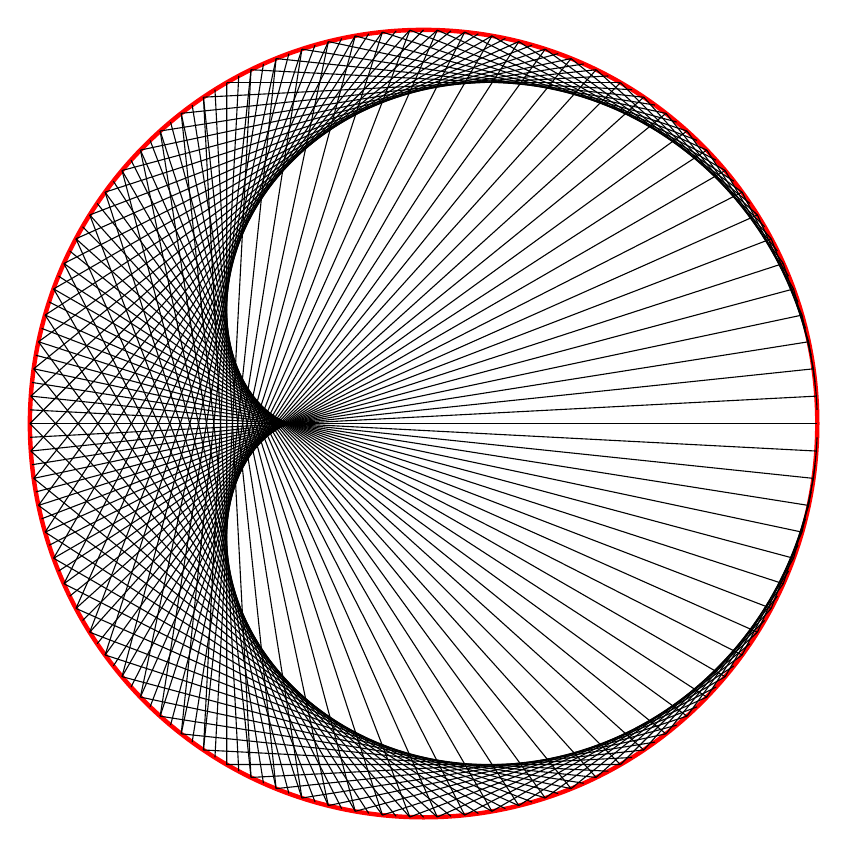
\begin{tikzpicture}

	\def\n{180}
	\def\r{5}
	\pgfmathsetmacro{\nm}{\n - 1}
	\def\c{2}

%	\foreach \i in {0, 1, ..., 3}
%		\filldraw[red] ( 5*cos(\i*360/\n), 5*sin(\i*360/\n) ) circle (2pt);
		
%	\foreach \i in {0, 1, ..., 3}
%		\draw (\i, \pgfmathsin{\i r}) circle (2pt);
	
	\draw[red, ultra thick] circle (\r cm);
	
	\foreach \i in {0, 1, ..., \nm}
		{
			\pgfmathsetmacro{\x}{\r*cos(\i*2*pi/\n r)}
			\pgfmathsetmacro{\y}{\r*sin(\i*2*pi/\n r)}
			
			\pgfmathsetmacro{\p}{\r*cos(\i*2*\c*pi/\n r)}
			\pgfmathsetmacro{\q}{\r*sin(\i*2*\c*pi/\n r)}
			
%			\filldraw[red] (\x, \y) circle (1pt);
			\draw (\x, \y) -- (\p, \q);
		}
		
%	\foreach \x in {-3.141, -3.140, ..., 3.14}
%		{
%			\pgfmathsetmacro{\y}{sin(\x r)}
%			
%			\filldraw[black] (\x, \y) circle (.3pt);	
%		}
	

\end{tikzpicture}



\end{document}